\documentclass[11pt,a4paper]{article}
\usepackage[utf8]{inputenc}\usepackage[T1]{fontenc}\usepackage[english]{babel}
\usepackage[margin=2.7cm]{geometry}\usepackage{amsmath,amssymb,amsthm,mathtools}
\usepackage{graphicx,booktabs,tabularx,longtable,array,float}\usepackage{natbib}\usepackage{hyperref}
\hypersetup{hidelinks,pdfauthor={Brian Axel Rodriguez},pdftitle={The Wealth of Optionality}}
\graphicspath{{../figures/en/}}\setlength{\parindent}{1.1em}\setlength{\parskip}{0.18em}\setlength{\emergencystretch}{2em}
\newtheorem{theorem}{Theorem}[section]\newtheorem{proposition}[theorem]{Proposition}\newtheorem{corollary}[theorem]{Corollary}\newtheorem{definition}[theorem]{Definition}\newtheorem{assumption}[theorem]{Assumption}
\newcommand{\E}{\mathbb E}\newcommand{\R}{\mathcal R}\newcommand{\Prb}{\mathbb P}\newcommand{\dd}{\mathrm d}\newcommand{\1}{\mathbf 1}
\title{\textbf{The Wealth of Optionality: Liquidity, Financial Selection, and Shock Propagation in Production Networks}}
\author{Brian Axel Rodriguez\\\small Independent Research}\date{2026}
\begin{document}\maketitle
\begin{abstract}
Liquidity reserves buy time: they allow a firm to meet obligations, reorganize input sourcing, wait for receivables, or postpone an irreversible decision. This paper develops a theoretical framework for how this temporal margin may affect firm selection and shock propagation in production networks. First, it defines runway as resources usable within the horizon of obligations, without equating receivables with cash or uncommitted borrowing capacity with available credit. Under an explicit Lomax distribution for cash-flow shocks, it derives the probability of liquidity distress, its marginal sensitivity, and a measure of urgency. This functional form is conditional on the chosen distribution and is not presented as a universal law. Second, it shows how payment delays can reduce effective runway and amplify losses through a network, under explicit restrictions on monetization, substitution, and the stability of the propagation operator. Third, it characterizes when an aggregate representation by moments is exact and when a bin-based approximation admits error bounds. Exact moment closure requires omitted states—including relevant network links and fiscal or trade liabilities—not to alter transitions once aggregates are fixed. Fourth, it audits empirical identification: payment delays may affect liquidity and survival, but financial fragility may also change a firm’s payment behavior, credit access, and supplier selection. The included data describe accounting ratios for listed Argentine firms; they do not jointly observe invoices, realized payment dates, supplier-customer links, and firm exit. They therefore do not identify the mechanism causally. The contribution is an analytical structure with conditional results, verifiable closure conditions, and a testing strategy that separates theory, simulation, and observational evidence.
\end{abstract}
\noindent\textbf{Keywords:} liquidity runway; trade credit; firm selection; production networks; micro--macro closure; endogeneity.\\
\noindent\textbf{JEL codes:} C63, D22, D85, E23, G32, L14, L25.

\section{Introduction}
A firm may have orders, workers, and productive technology and still fail to reach the next period because wages, taxes, or inputs fall due before sales are collected. The difference between continuing operations and cutting production need not coincide with a productivity difference. It may depend on how long the firm can cover its commitments with resources that are actually accessible. This temporal margin is what we call \emph{runway}.

The idea does not replace theories of productivity, selection, or networks. It connects them through a short-run liquidity constraint. The corporate-liquidity literature emphasizes the precautionary value of cash when external finance is costly and future project value depends on available liquidity \citep{almeida2014,almeida2007,fazzari1988}. Production-network research shows that idiosyncratic shocks can propagate through specific inputs and production links \citep{acemoglu2012,carvalho2014,barrot2016}. Trade-credit research shows that interfirm obligations transmit financial stress and that supplier credit can act as a contingent source of liquidity \citep{boissay2013,jacobson2015,amberg2021,costello2020}. Studies combining production and financial networks find that financial constraints can amplify shocks originating outside the directly affected firm \citep{demir2024,huremovic2026}. These contributions motivate the mechanism; they do not prove that one parameterization describes every economy or that public payment delays are exogenous.

The paper’s contribution is deliberately bounded. (i) It derives a liquidity-risk function and a measure of urgency under an explicit shock distribution. (ii) It establishes conditions under which payment delays reduce runway and transmit losses to other firms. (iii) It formalizes exact moment closure and a distributional approximation bound. (iv) It distinguishes claims that can be proved analytically from those requiring numerical computation or microdata. (v) It examines endogeneity, reverse causality, simultaneity, and network effects before proposing an empirical strategy.

The paper does not claim a global bifurcation, general hysteresis, or an estimated causal effect. Numerical certificates associated with a reduced system do not automatically transfer to a field derived from microeconomic decisions. Likewise, a synthetic exercise that reproduces a trajectory is not empirical calibration. The narrower defensible thesis is that liquidity can alter which productive options remain feasible, and that the strength of this channel depends on technology, obligations, accessible credit, and network topology.

\section{Firm state and liquidity accounting}
Let $i$ denote an active firm in period $t$. Let $C_{it}$ be available cash; $L^u_{it}$ committed but undrawn credit; $\theta_{it}\in[0,1]$ the fraction usable within the relevant horizon; $F_{it}$ funds obtained through factoring or other effective monetization, net of any asset already recorded as transferred; $A^g_{it}$ public-sector receivables not yet collected or discounted; $B_{it}>0$ essential expenditure per unit of time; and $\omega_{it}\in[0,1]$ the fraction of public receivables that can be converted into liquidity within that horizon.

Define effective runway as
\begin{equation}
R_{it}=\frac{C_{it}+\theta_{it}L^u_{it}+F_{it}+\omega_{it}A^g_{it}}{B_{it}}. \label{eq:runway}
\end{equation}
The unit of $R$ is time when $B$ is expenditure per unit of time. The expression does not imply that the face value of an invoice is available cash: $\omega$ captures only monetization feasible before the relevant obligations fall due. If an invoice has already been factored, it must be excluded from $A^g$ to prevent double counting. Uncommitted credit, borrowing that a bank might provide in the future, and expected sales also do not belong in the numerator without an explicit access rule.

Runway is an indicator of short-term payment capacity, not a sufficient measure of solvency or an automatic prediction of survival. It does not by itself incorporate covenants, discrete maturities, customer concentration, collateral, closure costs, refinancing access, owner decisions, or heterogeneity in the timing of receipts and payments. Applications must measure or model these components separately.

Cash accounting obeys a stock-flow identity such as
\begin{equation}
C_{i,t+1}=C_{it}+\text{Receipts}_{it}+\text{New credit}_{it}-\text{Payments}_{it}-\text{Debt service}_{it}-\text{Taxes}_{it}+\text{Other flows}_{it}. \label{eq:cashflow}
\end{equation}
Receivables and payables must be updated consistently with realized flows. An increase in accounts receivable is not a cash receipt in the accrual period; an increase in accounts payable is trade financing and a future obligation, not operating income. This distinction matters because a model can generate artificially rising runway if accrued sales are accumulated as cash or if input expenditure, payroll, taxes, or debt repayment are omitted.

\section{From cash risk to urgency}
\subsection{General definition}
Let $X_i\geq0$ denote the unexpected cash loss accumulated over the relevant horizon. If accessible reserves equal $B_iR_i$, liquidity distress occurs when $X_i>B_iR_i$. The distress probability is
\begin{equation}
q(R)=\Prb(X>BR)=1-F_X(BR),\qquad R\geq0. \label{eq:qgeneral}
\end{equation}
If $X$ has a positive density $f_X$ over the relevant range, then $q'(R)=-Bf_X(BR)<0$. This property does not require a parametric distribution. The distribution determines tail shape, the rate at which risk falls, and extrapolation to extreme runway values.

\subsection{Lomax benchmark and analytical results}
For a closed-form benchmark, assume a Lomax cash-flow shock with scale $s>0$ and shape $\alpha>0$, whose survival function is $\Prb(X>x)=(1+x/s)^{-\alpha}$. Then
\begin{equation}
q_L(R)=\left(1+\frac{BR}{s}\right)^{-\alpha}. \label{eq:lomax}
\end{equation}
The Lomax distribution allows a power-law tail and a parsimonious representation of positive heavy-tailed losses. It does not follow from positivity of $X$: it is an assumption that should be compared with alternatives, including the lognormal, using tail quantiles, out-of-sample fit, and stability across sectors and periods.

\begin{proposition}[Urgency under a Lomax tail]
Under \eqref{eq:lomax}, the distress probability is decreasing and convex in $R$. In particular,
\begin{align}
-q'_L(R)&=\frac{\alpha B}{s}\left(1+\frac{BR}{s}\right)^{-\alpha-1}, \label{eq:marginal}\\
q''_L(R)&=\frac{\alpha(\alpha+1)B^2}{s^2}\left(1+\frac{BR}{s}\right)^{-\alpha-2}>0. \label{eq:convex}
\end{align}
The absolute elasticity of distress risk with respect to runway is
\begin{equation}
\eta_L(R)=-\frac{R q'_L(R)}{q_L(R)}=\frac{\alpha BR}{s+BR}. \label{eq:elasticity}
\end{equation}
\end{proposition}
\begin{proof}
Differentiating the survival function in \eqref{eq:lomax} once and twice gives \eqref{eq:marginal} and \eqref{eq:convex}. Multiplying $-q'_L/q_L$ by $R$ simplifies to \eqref{eq:elasticity}. The signs follow from $B,s,\alpha>0$.\end{proof}

Three objects must be distinguished. $q(R)$ is a probability; $-q'(R)$ is the marginal reduction in that probability from an additional unit of runway; $\eta(R)$ is an elasticity. An objective function could penalize expected distress, the cost of holding cash, or marginal avoided losses, but these magnitudes are not interchangeable. For example,
\begin{equation}
\mathcal C(R)=c_RR+c_Dq(R),\qquad c_R,c_D\geq0, \label{eq:cost}
\end{equation}
expresses an illustrative trade-off between the cost of liquidity and expected distress costs. It is not, by itself, an equilibrium condition and does not identify $c_R,c_D,s,\alpha$.

\begin{figure}[htbp]\centering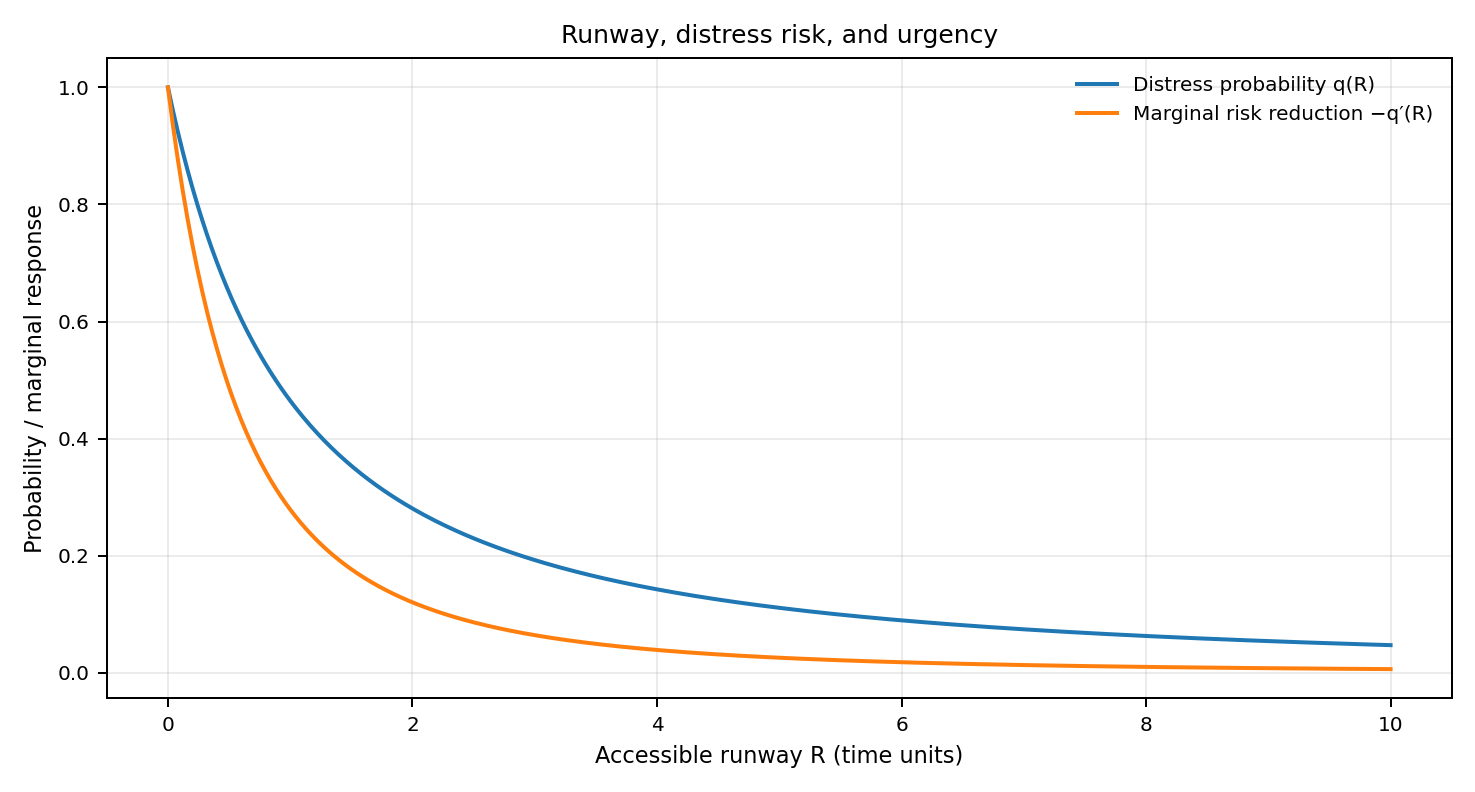
\includegraphics[width=.78\linewidth]{runway_urgency.png}\caption{Distress probability and marginal risk reduction under a Lomax distribution. Parameters are illustrative, not estimated.}\label{fig:runway}\end{figure}

\section{Optionality and the firm’s dynamic decision}
Runway matters economically because it changes the set of actions a firm can finance until the next adjustment opportunity. Let $a\in\mathcal A$ be an action—continue, invest, innovate, substitute a supplier, or wait—and let $c(a)$ be its cash requirement over the relevant horizon. For a state with runway $R$, define the feasible set
\begin{equation}
\mathcal A(R)=\{a\in\mathcal A:c(a)\leq BR+M(a)\},
\end{equation}
where $M(a)$ includes only inflows or financing verifiably available for that action. If $R_2\geq R_1$ and other conditions are unchanged, then $\mathcal A(R_1)\subseteq\mathcal A(R_2)$. Liquidity can expand the menu of decisions even if it does not directly change technological productivity.

\begin{definition}[Value of optionality]
Let $U(a,s)$ be the value of action $a$ in state $s$. The static value of optionality is $V(R,s)=\sup_{a\in\mathcal A(R)}U(a,s)$. The optionality gain between two runway levels is $\Omega(R_2,R_1;s)=V(R_2,s)-V(R_1,s)$ for $R_2\geq R_1$.
\end{definition}

\begin{proposition}[Monotonicity of optionality]
If the feasible action set is nested in runway and action payoffs do not mechanically change with $R$, then $V(R,s)$ is nondecreasing in $R$ and $\Omega(R_2,R_1;s)\geq0$.
\end{proposition}
\begin{proof}
Since $\mathcal A(R_1)\subseteq\mathcal A(R_2)$, the supremum of $U(a,s)$ over the second set cannot be lower than the supremum over the first.\end{proof}

In a dynamic problem, continuation value can be written as
\begin{equation}
V(s)=\max\left\{0,\sup_{a\in\mathcal A(R(s))}\left[u(s,a)+\beta\E\left(V(s')\mid s,a\right)\right]\right\}, \label{eq:bellman}
\end{equation}
where zero represents exit. The equation defines the object but does not solve it: a solution requires states, laws of motion, payoffs, credit constraints, shock distributions, and boundary conditions to be specified. Static monotonicity also does not guarantee that more cash increases realized innovation in every model. A firm may hold cash, repay debt, or distribute dividends; an available option need not be chosen; and the cost of financing reserves may change with runway. The proposition is therefore a feasibility result, not a universal prediction about investment or productivity.

The connection to firm selection requires separating productivity, liquidity, and entry. Classic industrial-dynamics models show that heterogeneity, learning, entry, and exit shape the long-run firm distribution \citep{jovanovic1982,hopenhayn1992}; in trade, reallocation across firms contributes to aggregate productivity \citep{melitz2003}. The extension considered here is that financial capacity may change which firms survive a shock and which options they retain, conditional on productivity. The paper does not claim that liquidity replaces productivity or that financial selection always dominates.

For an open population, a general law of motion is
\begin{equation}
\mu_{t+1}=\mathcal T(\mu_t;\vartheta_t)-\mathcal X(\mu_t;\vartheta_t)+\mathcal B(\mu_t;\vartheta_t),
\label{eq:openpopulation}
\end{equation}
where $\mathcal T$ redistributes active mass across states, $\mathcal X$ records exits, and $\mathcal B$ entries. Internal transitions must conserve mass; active mass changes only through entry and exit. This accounting prevents entry from being treated as a disconnected appendix to the existing distribution. However, writing \eqref{eq:openpopulation} does not prove existence of a long-run equilibrium, uniqueness of a stationary distribution, or hysteresis. Those results depend on entry rules, expected profits, sunk costs, productivity transitions, and the network.

\subsection{A minimal microfoundation for continuation value}
To make the Bellman equation operational, separate technology from financial conditions. Let $s=(z,R,d,g,a)$, where $z$ is productivity, $R$ effective runway, $d$ net debt, $g$ the commercial-network state, and $a$ age or experience. An action $u$ includes production, investment, innovation, trade-credit payments, and exit. The transition is a distribution $P(\dd s'\mid s,u,\varepsilon)$ in general. The active firm's problem is
\begin{equation}
V(s)=\max\left\{V^{\mathrm{exit}}(s),\sup_{u\in\Gamma(s)}\left[\pi(s,u)-\chi(u)+\beta\int V(s')P(\dd s'\mid s,u)\right]\right\}.
\label{eq:bellman_micro}
\end{equation}
Here $\Gamma(s)$ is the feasible action set, $\pi$ net operating flow, $\chi$ an adjustment cost, and $V^{\mathrm{exit}}$ liquidation value net of obligations. The financial constraint must enter $\Gamma(s)$ or the cash transition; it is not enough to include $R$ as a covariate in an exit probability. If an action requires payment $m(u)$ before revenues arrive, a minimal constraint is $m(u)\leq C+\theta L^u+F+\omega A^g$, adjusted for obligations falling due in the same horizon.

This is a microfoundation template, not a computed solution. A well-posed problem requires a state/action space, transition laws for productivity, cash, debt and contracts, a pricing or demand rule, default and liquidation conventions, an entry rule, and integrability conditions. Without these elements, one cannot invoke a contraction theorem to claim existence and uniqueness of the value function.

\begin{proposition}[Value monotonicity under nested feasibility]
Consider two states that differ only in liquid resources, $s_1$ and $s_2$, with $R_2\geq R_1$. If $\Gamma(s_1)\subseteq\Gamma(s_2)$, payoffs and transition distributions for common actions are identical, and exit value does not fall, then $V(s_2)\geq V(s_1)$.
\end{proposition}
\begin{proof}
Every action feasible in $s_1$ is feasible in $s_2$ and has the same continuation value. The supremum over the larger set therefore cannot be smaller, and the exit option does not reduce the maximum.\end{proof}

The identical-transition assumption matters. If additional cash changes opportunity costs, collateral, credit prices, irreversible investment, or contractual terms, payoffs or transitions differ and monotonicity does not follow from nested feasibility alone. Nor does the proposition make observed cash exogenous: firms with better opportunities may accumulate cash, while firms anticipating adverse shocks may hoard it.

\subsection{Entry and selection as equilibrium conditions}
Exit can be represented by a stopping rule $\tau_e=\inf\{t:V^{\mathrm{continue}}(s_t)\leq V^{\mathrm{exit}}(s_t)\}$. A stylized free-entry condition requires expected entrant value net of sunk cost $k_e$ to be nonpositive:
\begin{equation}
\mathbb E[V(s_0)\mid \text{entry}]-k_e\leq0,
\end{equation}
with equality under interior entry. This condition cannot be evaluated without specifying entrants' state distribution and the effects of entry on prices, demand and networks. A computational rule that randomly replaces some exiting firms is not free entry and does not prove a stationary distribution.

For any measurable set $A$ of active states, mass accounting requires
\begin{equation}
\mu_{t+1}(A)=\int P(s,A\mid s,u^*(s),G_t)\,\mu_t(\dd s)+\nu_{t+1}(A)-\xi_{t+1}(A),
\label{eq:mass_balance}
\end{equation}
where $\nu$ is entrant mass and $\xi$ is exiting mass. Stationarity would require $\mu_{t+1}=\mu_t$ together with consistent entry, prices and networks; it does not follow from bounding population size by construction.

\subsection{What micro--macro closure requires}
Closure is not established by choosing a few moments and simulating their transitions. Let $S(\mu,G,\ell)$ denote aggregate statistics and auxiliary states. Exact closure requires any two microstates with identical aggregates to yield identical next-period aggregates. Equivalently, for all $x_1,x_2$ with $S(x_1)=S(x_2)$,
\begin{equation}
S(\mathcal T(x_1))=S(\mathcal T(x_2)).
\label{eq:fiber_test}
\end{equation}
This condition is falsifiable: construct microstates with equal mean cash, mean productivity and active mass but different runway dispersion, customer concentration or maturity profiles. Different next-period aggregates reject the proposed closure. A network cannot be omitted when transitions depend on exposures not determined by the retained aggregates; mean degree is insufficient if outcomes depend on centrality, flow direction, or correlation between fragility and network position.

Bin approximation is a numerical step after closure, not a closure proof. Report separately (a) within-bin distribution representation error, (b) induced aggregate-field error, (c) time-integration error, and (d) network approximation error. A Gronwall bound controls trajectory error only after a uniform field-error bound and a valid Lipschitz constant on a common invariant region have been established. Discrete state changes, exit discontinuities and network rewiring require additional arguments.

\subsection{Distributional closure versus finite-moment closure}
A precise closure statement must specify the level of aggregation. Let the complete firm state be
\[
x_i=(c_i,d_i,\ell_i,r_i,\mathbf a_i,z_i,k_i,n_i,\tau_i),
\]
where the coordinates record cash, debt, usable credit, inventories, the vector of receivables/payables by maturity, productivity, productive capacity, input requirements, and contract/payment status. Let $G_t$ be the directed weighted supplier graph, and let $\mathfrak M_t=(N_t,(x_i)_{i\leq N_t},G_t,\ell_t^A)$ include population size and any aggregate prices or fiscal states needed by individual decisions. The notation deliberately retains the full labeled network: a marginal distribution of firm states alone does not generally preserve who trades with whom.

\begin{assumption}[Complete-state Markov sufficiency]
Conditional on $\mathfrak M_t$, the law of exogenous shocks is specified; each active firm's decision rule depends only on its state and the included aggregate/network state; entry and exit kernels are specified; and network rewiring and aggregate-price updates are governed by specified transition kernels. No omitted history variable affects these conditional laws.
\end{assumption}

\begin{theorem}[Distributional micro--macro closure]
Under complete-state Markov sufficiency, there exists a transition kernel $\mathcal P$ such that
\[
\Pr(\mathfrak M_{t+1}\in A\mid\mathfrak M_0,\ldots,\mathfrak M_t)=\mathcal P(A\mid\mathfrak M_t)
\]
for every measurable set $A$. Thus the full population-and-network state is Markov and closes exactly in distribution. This result does not imply that a finite vector of moments, or the runway distribution alone, is a sufficient state.
\end{theorem}

\begin{proof}[Proof sketch]
By assumption, conditional on the current complete state, each decision, idiosyncratic shock, entry/exit event, network update, and aggregate-state update has a specified conditional law that does not depend on earlier history. Their joint conditional law therefore determines the distribution of the next complete state as a function of $\mathfrak M_t$ alone. Integrating over the specified shocks yields the transition kernel $\mathcal P$. If an omitted maturity, inventory, contract, price, or network-history variable changes one of those conditional laws, the assumption fails and the proposed state is not closed.
\end{proof}

This theorem supplies a clean micro--macro closure at the full-state distributional level, not a solved equilibrium or a finite-dimensional reduction. It also identifies the burden of proof for a smaller aggregate state: one must show that its fibers are invariant under the next-period aggregate law. The current ABM closes only its own programmed rule system; it does not yet contain the richer inventories, complementary-input technology, endogenous prices, and contractual states needed to claim closure of the economic mechanism in full.

\subsection{Consistency audit of the agent-based laboratory}
The simulator has been revised so that current-period inputs must be financed before production and realized sales are scaled by the share of planned inputs actually purchased. This removes the previous logical inconsistency in which input rationing affected exit but left contemporaneous sales unchanged. The proportional mapping is still a stylized quantity constraint, not an estimated production technology: inventories, multiple complementary inputs, capacity utilization, and endogenous input prices are not fully modeled. The ABM is therefore a mechanism laboratory, not a calibrated production-network model, and its outputs do not identify a causal productivity elasticity with respect to payment delays.

The remaining audit should test period-by-period cash and debt identities, conservation of buyer and supplier flows, boundary cases (zero delay, no public channel, empty network, abundant credit, and no shocks), global sensitivity, and out-of-sample moments. Dynamic calibration remains unsuccessful and should be reconsidered only after those identities and transition rules have been verified; otherwise parameter tuning would confound structural misspecification with parameter error.

\subsection{Lognormal alternative and functional robustness}
An alternative specification uses a lognormal tail. If $\ln X\sim N(m,\sigma^2)$, with $R>0$, define $z(R)=[\ln(BR)-m]/\sigma$. Then
\begin{equation}
q_{LN}(R)=\overline\Phi(z(R)),\qquad -q'_{LN}(R)=\frac{\phi(z(R))}{\sigma R},\qquad -\frac{Rq'_{LN}(R)}{q_{LN}(R)}=\frac{\phi(z(R))}{\sigma\overline\Phi(z(R))}. \label{eq:lognormal}
\end{equation}
The last expression is the inverse Mills ratio scaled by $1/\sigma$. Unlike the Lomax, the lognormal does not impose a power-law tail. Neither distribution is identified by shock positivity; selection should be based on tail fit, out-of-sample stability, and the economic relevance of the risk horizon. The closed-form results above are therefore conditional comparative statics, not a claim about a universal distribution of firm losses.

\section{Payment delays and network propagation}
\subsection{Direct effect on runway}
Suppose public payment delay is $\tau$ and timely monetization of invoices satisfies $\omega'(\tau)\leq0$. Holding the other components of \eqref{eq:runway} fixed,
\begin{equation}
\frac{\partial R_i}{\partial\tau}=\frac{A_i^g}{B_i}\omega_i'(\tau)\leq0. \label{eq:dRdtau}
\end{equation}
Define $h_i(R)=h_0+\kappa q(R)$ with $h_0,\kappa\geq0$ and $h_0+\kappa\leq1$. Since $0<q(R)\leq1$, this parameter restriction ensures $h_i(R)\in[0,1]$ for every $R\geq0$. Then $\partial h_i/\partial\tau=\kappa q'(R_i)\partial R_i/\partial\tau\geq0$. This sign is a conditional implication of the exposure definition, not an empirical estimate. It can vanish if the invoice is fully discounted, expenses do not fall due before collection, the supplier substitutes the buyer, or offsetting cash inflows coincide with the delay.

\begin{proposition}[Comparative statics of delay]
If $A_i^g/B_i\geq0$, $\omega_i'(\tau)\leq0$, $q'(R)<0$, $h_0,\kappa\geq0$, and $h_0+\kappa\leq1$, then a longer delay does not increase runway and does not reduce the exit hazard: $\partial R_i/\partial\tau\leq0$ and $\partial h_i/\partial\tau\geq0$.
\end{proposition}
\begin{proof}
The first inequality follows from \eqref{eq:dRdtau}. For the second, apply the chain rule to the hazard and multiply two non-positive derivatives: $\kappa q'(R_i)\partial R_i/\partial\tau\geq0$.\end{proof}

\subsection{Supplier networks and propagation stability}
Let $W$ be a nonnegative payment-network exposure matrix, where $W_{ij}$ is the share of supplier $i$’s sales accounted for by customer $j$. Let $u\geq0$ be the vector of direct liquidity losses. A local linear approximation to successive transmission rounds is
\begin{equation}
x=u+\beta Wx,\qquad x=(I-\beta W)^{-1}u, \label{eq:network}
\end{equation}
provided the spectral radius satisfies $\rho(\beta W)<1$. Under this condition the Neumann series converges and
\begin{equation}
x=\sum_{k=0}^{\infty}(\beta W)^ku\geq u. \label{eq:neumann}
\end{equation}
The inequality is componentwise and follows from non-negativity of $W$. The inverse is a \emph{frozen-network, short-run equilibrium multiplier}: it holds the active set, exposure matrix, and local response coefficient fixed, before exit thresholds, supplier switching, or contract renegotiation are activated. It shows how a direct loss can trigger additional rounds within that local regime; it does not imply that all firms face the same effect or that a linear multiplier remains valid when firms exit, change suppliers, or renegotiate contracts endogenously.

Substitutability reduces effective exposure. One illustrative parameterization is $\widetilde W_{ij}=W_{ij}(1-\sigma_{ij})$, with $\sigma_{ij}\in[0,1]$. Without data on substitution, purchase concentration, and commercial links, $\sigma$ cannot be identified from aggregate balance sheets. If used to identify spillovers, the exposure matrix should be constructed from relationships that predate the shock; the contemporaneous network may itself be an outcome of financial stress.

\subsection{Working-capital constraints and realized production}
A minimal link between cash and production separates potential from realized output. Let $y_i^*=A_i k_i^{\alpha}l_i^{\gamma}$ be potential production, with $\alpha,\gamma\geq0$ and $\alpha+\gamma\leq1$. If production requires an intermediate input $m_i$ per unit, the physical constraint is $y_i\leq m_i/\nu_i$, where $\nu_i>0$ is the unit requirement. If the input must be paid for before sale, liquid resources constrain purchases:
\begin{equation}
 m_i\leq \frac{C_i+\theta_iL_i^u+F_i+\omega_iA_i^g-\mathcal O_i}{p_i^m},\qquad
 y_i=\min\left\{y_i^*,\frac{m_i}{\nu_i}\right\},
\label{eq:working_capital_prod}
\end{equation}
where $\mathcal O_i$ denotes other obligations due before sale and $p_i^m$ is the input price. This is illustrative: with multiple complementary inputs, the binding constraint is the minimum across required inputs; inventories, supplier credit and partial payments require a richer intertemporal transition.

The equation explains why observed sales must not be equated with productivity. Lower output may result from lower $A_i$, less capital or labor, or an input that could not be financed. Nominal sales also mix quantities and prices. Measuring firm productivity requires real output and input measures, treatment of markups and capacity utilization, and attention to exit selection; those variables are not available as a linked panel here.

Network propagation can be introduced by making input availability $m_i$ depend on deliveries from suppliers $j$, which in turn depend on their own cash constraints. The transition is simultaneous or sequential depending on the timing of production, delivery and payment. If deliveries are determined before sales, working-capital constraints can generate a quantity effect; if suppliers deliver on credit, the immediate channel may operate through payables before affecting production. Timing is not a programming detail: it determines which shocks propagate within a period and which propagate with a lag.

\section{Firm distributions, closure, and bin approximation}
\subsection{Distributional law}
Let $s$ be the firm state and $G$ its commercial graph. Let $\mu_t$ be the measure over active states and $T_t$ the transition operator combining decisions, shocks, routine switching, entry, and exit. The exact joint law of population and network transitions is $(\mu_{t+1}, G_{t+1}) = T_t(\mu_t, G_t)$. Aggregates are obtained through a map $S(\mu_t,G_t,\ell_t)$ that may include active mass, runway distribution, productivity, debt, payables, and network structure.

\begin{definition}[Exact moment closure]
The aggregate system closes exactly with respect to $S$ if there exists an operator $\Phi$ such that $S(T(\mu, G)) = \Phi(S(\mu, G))$ for all admissible states and network structures, natively incorporating the post-transition graph generated by the economic transition.
\end{definition}

\begin{theorem}[Necessary and sufficient condition for closure]
For a joint transition $T$ and aggregate map $S$, a function $\Phi$ satisfying $S(T(\mu, G)) = \Phi(S(\mu, G))$ exists on the domain if and only if $S(T(\mu_1, G_1)) = S(T(\mu_2, G_2))$ whenever $S(\mu_1, G_1) = S(\mu_2, G_2)$. Equivalently, the mapping $S \circ T$ must be constant on every fiber of $S$.
\end{theorem}
\begin{proof}
If $\Phi$ exists, two state-network configurations $(\mu_1, G_1)$ and $(\mu_2, G_2)$ with the same aggregate value $S$ have the same image under $S \circ T$ by direct substitution. Conversely, if $S \circ T$ is constant on each fiber, define $\Phi(s) = S(T(\mu, G))$ for any pair $(\mu, G)$ such that $S(\mu, G) = s$. This condition makes the definition strictly independent of the representative configuration selected from the fiber.
\end{proof}

The economic implication is important: the marginal runway distribution is not enough if two firms with the same runway face different contracts, suppliers, liabilities, or substitution possibilities that alter future transitions. The minimum state must include variables that change future decisions. This is consistent with the heterogeneous-agent and aggregation literature, where closure by a few moments is a property of a model class rather than a universal identity \citep{krusell1998,achdou2022}.

\subsection{Projection bound}
Suppose $f$ is Lipschitz in runway with constant $L_f$, and every bin $B_k$ has diameter at most $\Delta$. For a probability measure $\mu$ and representative $r_k\in B_k$, define $\widehat I=\sum_k f(r_k)\mu(B_k)$.
\begin{proposition}[Bin integration error]
Under these assumptions,
\begin{equation}
\left|\int f(R)\,\dd\mu(R)-\sum_k f(r_k)\mu(B_k)\right|\leq\frac{L_f\Delta}{2}, \label{eq:binbound}
\end{equation}
when $r_k$ is the midpoint of each bin.
\end{proposition}
\begin{proof}
For every $R\in B_k$, $|f(R)-f(r_k)|\leq L_f|R-r_k|\leq L_f\Delta/2$. Integrate over each bin, sum, and use $\sum_k\mu(B_k)=1$.\end{proof}

The integration bound is not a bound on dynamic-field error. For trajectory approximation, additionally suppose fields $F$ and $F_K$ are Lipschitz with common constant $L$ on a common invariant region and $\sup_x\|F(x)-F_K(x)\|\leq\delta_K$. If $x(0)$ and $x_K(0)$ are initial states, Grönwall’s inequality implies
\begin{equation}
\|x(t)-x_K(t)\|\leq e^{Lt}\|x(0)-x_K(0)\|+\frac{\delta_K}{L}(e^{Lt}-1),\quad L>0. \label{eq:gronwall}
\end{equation}
The bound applies only in a local regime where the active set of firms remains fixed over the bounded time window; discrete firm exit or network rewiring can make the vector field discontinuous or only piecewise Lipschitz. The proof follows from the integral inequality for trajectory differences and Grönwall’s lemma. The bound requires a field-error bound, a common region, and Lipschitz regularity; it does not automatically certify a bin algorithm. Nor does it certify stationary roots, stability, folds, or hysteresis. Those claims require field and Jacobian errors, branch searches, and, when rigorous existence is asserted, interval verification of the specific system.

\subsection{Heterogeneity: why mean runway is insufficient}
The runway distribution matters even when the outcome of interest is expected distress alone. Under the Lomax benchmark and common burn $B$, $q_L(R)=(1+BR/s)^{-\alpha}$ is strictly convex for $R\geq0$, since
\begin{equation}
q_L''(R)=\alpha(\alpha+1)\left(\frac{B}{s}\right)^2\left(1+\frac{BR}{s}\right)^{-\alpha-2}>0.
\end{equation}
Jensen's inequality therefore implies, for a runway distribution with finite mean,
\begin{equation}
\mathbb E[q_L(R)]\geq q_L(\mathbb E[R]),
\label{eq:jensen_distress}
\end{equation}
strictly if runway is non-degenerate. Replacing a heterogeneous distribution with its mean thus understates expected distress under this specification. This is not a causal effect of financial inequality; it is a mathematical implication of the curvature of the risk function. With heterogeneous burn $B_i$, the inequality does not apply directly to mean $R_i$; the joint distribution of $B_iR_i$ or of reserves relative to obligations must be evaluated.

Distributional composition also matters. Transferring cash from a high-runway firm to a low-runway firm may reduce total risk if the recipient has a larger marginal distress reduction and transfers have no costs. But this depends on a common measurement horizon and frictionless reallocation. Cash trapped in subsidiaries, specific collateral, regulation, or creditor covenants may prevent transfers. Jensen's inequality motivates retaining dispersion and tails in the aggregate state; it does not prescribe a redistribution policy without modeling constraints.

An empirical decomposition should report means, medians, lower quantiles, mass near zero, and heterogeneity by sector and size in addition to aggregate ratios. Firms with high cash may also face high near-term obligations, so average cash/assets is not average runway. Numerator and denominator must be constructed from consistent accounting items, and averages of ratios should be reported with their denominators. These choices affect calibration and the interpretation of moments used in indirect inference.

\section{Indirect inference and the information content of moments}
If firm-level data and a fully specified simulator are available, indirect inference can estimate structural parameters $\vartheta$ by comparing observed moments with those generated by the model \citep{gourieroux1993}. Let $m_D$ be the vector of data moments and $m_S(\vartheta)$ the vector of simulated moments. A distance estimator is
\begin{equation}
\widehat\vartheta=\arg\min_{\vartheta\in\Theta}[m_D-m_S(\vartheta)]'W[m_D-m_S(\vartheta)],\qquad W\succeq0. \label{eq:indirect}
\end{equation}
The formula does not produce identification by itself. Moments must respond differentially to parameters, and the Jacobian $J(\vartheta)=\partial m_S(\vartheta)/\partial\vartheta'$ must have full column rank locally for regular local identification. If two parameters shift the same moments in similar ways, the objective may contain a flat valley and estimation will be weakly identified.

Moment selection should match the theoretical channels. Runway quantiles inform the distribution of accessible resources and expenditure; delay frequency and duration inform the payment process; the relation between direct shocks and supplier losses informs network propagation; and exit conditional on productivity and liquidity informs selection. Aggregate GDP or TFP moments cannot replace payment and network moments because they do not separate these channels. DSO and DPO can describe working capital but are not realized due and payment dates.

Indirect inference should incorporate sampling uncertainty, measurement error, and variation across simulation seeds. It should also be evaluated on moments not used in fitting and on held-out periods or firms. Recovering known parameters from synthetic data verifies that an algorithm can work under the specified data-generating process; it does not establish that the same parameters are identified in real data. At present, this equation is a protocol rather than an executed structural estimate.

\section{Limits of public data and diagnosis of available datasets}
The Yahoo Finance accounting pilot contains 537 reports for 52 listed Argentine firms between October 2021 and August 2026. The purported multi-country consolidation was audited and found structurally identical to the Argentina file; it was therefore excluded as an international sample. The analysis is restricted to the descriptive pilot of 52 listed Argentine firms. There are 240 annual and 297 quarterly rows, with temporal overlap; quarterly observations are concentrated in 2025--2026 and part of 2026 is incomplete. The frequencies should not be stacked as independent observations.

In the annual nonfinancial sample, the audited file contains 173 valid strict-runway observations: median 25.37 days, 10th percentile 4.43, and 90th percentile 93.49. Median DSO is 36.89 days and median DPO 61.80 days. These are unweighted row-level statistics, not firm-weighted statistics. Listed firms are not representative of unlisted firms, and firms that exited before reporting are missing. DPO has line-item mapping warnings; extreme values require tracing to source accounts rather than automatic deletion. The runway measure also does not automatically include committed credit, maturity schedules, future receipts, or non-operating payments.

The pilot does not observe invoice identifiers, contractual due dates, actual payment dates, buyers or suppliers, public contracts, or realized firm exit. It therefore cannot measure predetermined exposure to public arrears or reconstruct spillovers. Enterprise Surveys may describe establishments and questions on public contracts or payment delays, subject to the questionnaire, sampling design, and weights; a public frequency table is not equivalent to microdata ready for estimation. No firm-level regression is reported here.

In addition, the catalogue and public frequency table from the World Bank Enterprise Survey for Argentina describe questions on public contracts and payment timing. The documentation reports 797 establishments in the catalogue; 111 with a recent public contract (J.42); and 108 numeric responses on days to receive payment under such contracts (J.43). The unweighted mean is 62.7 days, the median 60, and the 90th percentile 109.5; 22.2\% of numeric responses report at least 90 days, with a maximum of 300. These values come from public frequencies, not a regression using downloaded microdata. They should not be interpreted as a causal estimate or as verified representativeness without checking survey weights, design, and special codes \citep{wbes2026}.

\begin{table}[htbp]\centering\small
\caption{Payments under public contracts in the WBES Argentina frequency table}
\begin{tabular}{lr}\toprule
Indicator & Value \\\midrule
Establishments in catalogue & 797 \\
With a recent public contract (J.42) & 111 \\
Numeric responses to J.43 & 108 \\
Unweighted mean days & 62.7 \\
Median days & 60 \\
90th percentile days & 109.5 \\
Responses with at least 90 days & 22.2\% \\
Maximum shown in the frequency table & 300 \\\bottomrule
\end{tabular}
\end{table}

\begin{figure}[htbp]\centering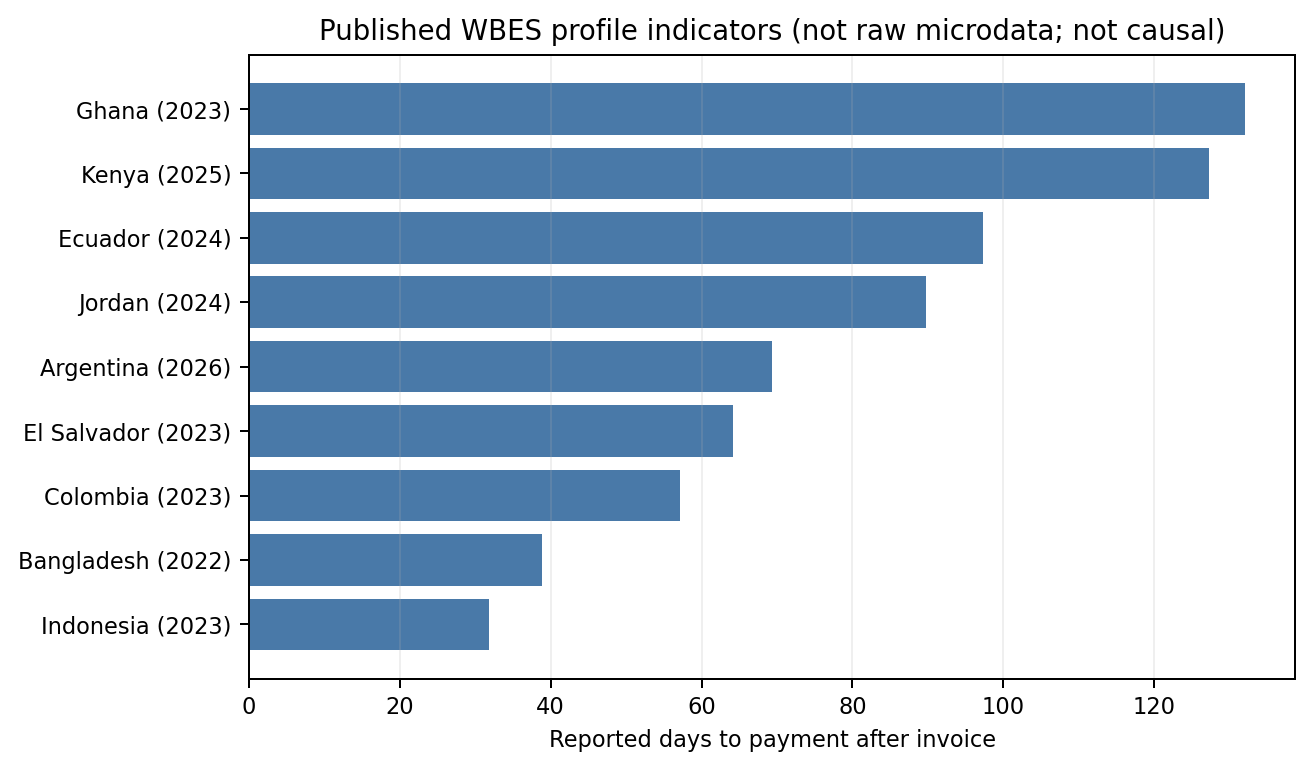
\includegraphics[width=.78\linewidth]{Fig10_WBES_payment_lags_EN.png}\caption{Public frequency-table distribution of reported payment times for public contracts in the Argentina Enterprise Survey. The chart is descriptive; it is not a weighted microdata estimate or a causal estimate.}\label{fig:wbeslags}\end{figure}

\begin{figure}[htbp]\centering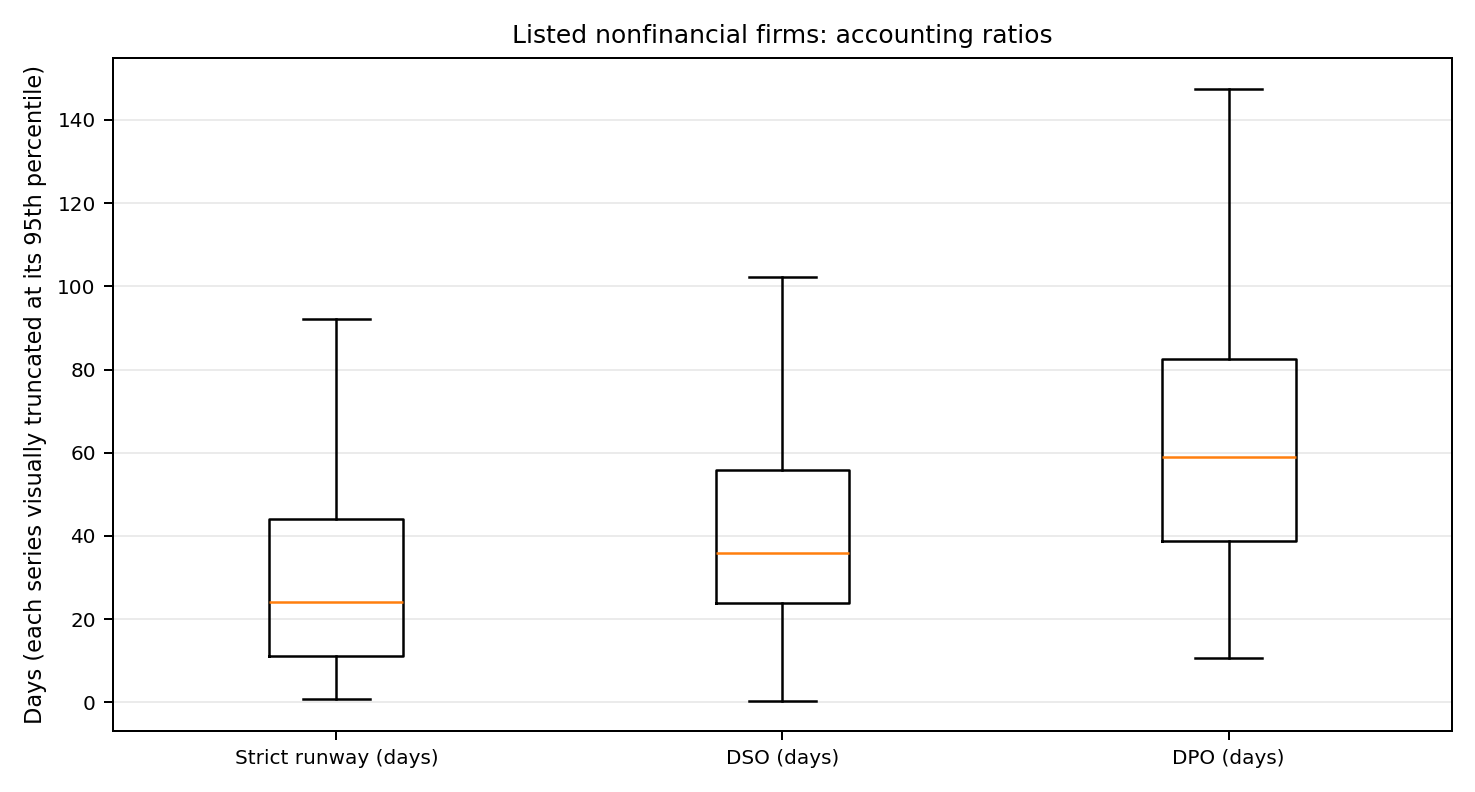
\includegraphics[width=.78\linewidth]{listed_firm_liquidity.png}\caption{Accounting-ratio pilot for listed Argentine firms. Series are visually truncated at their 95th percentile; the figure is descriptive, not representative, and does not identify public payments or production links.}\label{fig:pilot}\end{figure}

\section{Endogeneity, reverse causality, and identification}
\subsection{The problem has several components}
The relationship of interest connects delay by a public payer $\tau^g_{it}$, runway $R_{it}$, the firm’s own delay to suppliers $\delta^s_{it}$, outcomes $Y_{it}$, and survival $S_{it}$. These are distinct variables: $\tau^g$ measures how long the government takes to pay an obligation to the firm; $\delta^s$ measures how late the firm pays its own suppliers. A minimal structural representation is
\begin{align}
R_{it}&=r(\tau^g_{it},C_{it},L^u_{it},B_{it},A^g_{it},Z_{it}),\\
Y_{i,t+1}&=g(R_{it},A_{it},K_{it},N_{it},\varepsilon_{it}),\\
\delta^s_{it}&=d(R_{it},A^p_{it},\text{liquidity}_{it},\text{bargaining power}_{it},\nu_{it}),\\
\tau^g_{it}&=d(F_{it}^{\mathrm{fiscal}},Q_{it}^{\mathrm{admin}},\text{contract performance}_{it},\zeta_{it}),\\
N_{i,t+1}&=n(N_{it},Y_{it},\delta^s_{it},\xi_{it}),
\end{align}
where $F^{\mathrm{fiscal}}$ summarizes public-payer constraints, $Q^{\mathrm{admin}}$ contract administration, $A^p$ represents private sector accounts receivable, and $N$ production relationships. This representation is not estimated with the available data; it organizes sources of simultaneity.

First, public payment delay may create a cash-flow gap that leads the firm to delay its own supplier payments. Second, reverse causality may operate because delivery, documentation, quality, or solvency problems affect certification of a public invoice, while fragility may also increase $\delta^s$. Third, common shocks—recession, inflation, fiscal stress, regulatory changes, or sectoral conditions—can affect both $\tau^g$ and outcomes. Fourth, the network is endogenous: firms may switch suppliers, concentrate purchases, or lose customers in response to the same shock. Fifth, sample selection matters: financial statements observe listed firms that survive long enough to report and do not adequately capture entry and exit in the full firm population.

Recent evidence on firms delaying payments to their suppliers emphasizes that such behavior can reflect both financial flexibility and distress, and that realized payment records reveal patterns that aggregate balance sheets alone cannot recover \citep{wu2026,hirshleifer2019}. This literature informs the propagation channel but should not be confused with direct evidence on government delays in paying contractors; a delay should therefore not be treated as exogenous or as a unique indicator of fragility.

\subsection{Estimand and sources of non-identification}
The estimand must be chosen before selecting an estimator: the total effect of delay on survival, the effect mediated by liquidity, and the response of suppliers exposed to affected customers are distinct objects. A conventional firm-and-time fixed-effects panel coefficient would not identify a causal effect if public payment delay is correlated with unobserved shocks, if contract performance affects certification or payment timing, or if controls include post-treatment variables. Fixed effects remove time-invariant heterogeneity, not time-varying confounding or simultaneity. Controlling for contemporaneous runway may block the mediation channel under study; measurement error can introduce further bias. Given the current data, the paper therefore moves directly to potential outcomes and design requirements rather than presenting a conventional panel regression as an empirical candidate.

\subsection{Potential outcomes, network exposure, and estimands}
Let $D_i$ denote a pre-specified exposure to a payment-delay event and $Y_i(d,g)$ the outcome for firm $i$ under own exposure $d$ and network exposure $g$. With interference, the conventional potential outcome $Y_i(d)$ is incomplete: outcomes may depend on whether customers or suppliers are exposed. A direct effect at fixed network exposure is $\tau_D(g)=\mathbb E[Y_i(1,g)-Y_i(0,g)]$; a spillover effect at fixed own exposure is $\tau_G(d)=\mathbb E[Y_i(d,g_1)-Y_i(d,g_0)]$. These are distinct estimands and require an exposure mapping that summarizes the relevant network paths. If the mapping omits important counterparties, the estimand is not well-defined for the observed data.

A panel event-study specification might take the form
\begin{equation}
Y_{it}=\alpha_i+\lambda_{st}+\sum_{k\ne-1}\beta_k\,1[t-T_i=k]D_i^0+\sum_{k\ne-1}\gamma_k\,1[t-T_i=k]G_i^0+\varepsilon_{it},
\label{eq:event_study_network}
\end{equation}
where $D_i^0$ and $G_i^0$ are defined using pre-event contracts and network links, $T_i$ is the event date, $\alpha_i$ are firm effects and $\lambda_{st}$ are sector-by-time effects. This equation is a design template, not an estimated model. Its interpretation requires a credible event, no differential untreated trends conditional on the design, no anticipation beyond the modeled window, stable measurement, and a defensible treatment of staggered timing and heterogeneous effects. If treatment dates differ and effects are heterogeneous, a single two-way fixed-effect coefficient may combine comparisons with unintended weights; cohort-specific estimators and transparent aggregation are preferable.

The network exposure $G_i^0$ should be constructed before treatment, with sensitivity to radius, edge weights and direction. A direct shock to a government contractor can be propagated to upstream suppliers through its payment behavior, while a delay to the contractor's own public receivable is a separate exposure. The same firm can occupy both positions. The analysis should not collapse them into one scalar without stating the mapping. Standard errors must reflect both treatment assignment and network dependence; randomization inference or exposure-robust procedures may be needed where conventional clustering is inadequate.

\subsection{A possible design, not an executed estimate}
If a documented reform, operational change, or administrative regularization alters payment times in a plausibly exogenous way, one option is an event study with predetermined exposure:
\begin{equation}
Y_{it}=\alpha_i+\lambda_t+\sum_{k\neq-1}\beta_k\left(E_i^0\times\1\{t-T^*=k\}\right)+X_{it}'\gamma+u_{it}, \label{eq:eventstudy}
\end{equation}
where $E_i^0$ is exposure to public buyers measured before the event. A causal interpretation requires no anticipation, conditionally parallel trends, stable composition or appropriate corrections, no coincident differential shocks, and a transparent exposure definition. With staggered adoption or heterogeneous effects, appropriate estimators should be used instead of mechanically interpreting a conventional two-way fixed-effects regression \citep{callaway2021,sun2021,baker2026}.

An instrumental-variable strategy requires a variable $Z$ that changes payment timing but does not directly affect outcomes through other channels and is uncorrelated with unobserved shocks. An administrative rule or budget allocation is not a valid instrument merely because it precedes the outcome: it may affect public demand, investment, procurement quality, or expectations. The exclusion restriction and first stage require institutional justification and sensitivity tests. No instrument meeting these conditions has been verified here.

For spillovers, each supplier’s exposure should be constructed from pre-shock links, for example $E_i^{N,0}=\sum_j W^0_{ij}\tau^g_j$. Inference must allow interference across units: a control firm may be indirectly exposed to treated customers. Explicit exposure mappings, standard errors consistent with assignment, and falsification tests on links that should not transmit the shock are needed. The reflection problem in peer-interaction models and network simultaneity warn that correlations between peers do not automatically separate influence from selection or common shocks \citep{manski1993,bramoulle2009}.

\begin{table}[htbp]\centering\small
\caption{Identification threats and required responses}
\begin{tabularx}{\linewidth}{p{.23\linewidth}X X}\toprule
Threat & How it arises here & Required response \\
\midrule
Reverse causality & Firm fragility affects certification, its own payment behavior, credit, and supplier terms & Pre-shock covariates and network; institutional timing; defensible exogenous variation \\
Confounding & Fiscal stress, sectoral cycle, or inflation affects both delays and outcomes & Time/sector effects, pre-treatment controls, and justified comparability \\
Mediation & Runway mediates delay effects on outcomes & Distinguish total from direct effects; do not automatically control for mediators \\
Endogenous network & Firms switch suppliers after the shock & Freeze pre-treatment exposure and model interference \\
Selection & Listed firms and survivors differ from entrants and exits & Firm-population frame, exit tracking, and selection analysis \\
Measurement error & DSO/DPO and runway are not invoice dates or accessible cash & Link statements, invoices, due dates, realized payments, and committed credit \\
\bottomrule\end{tabularx}\end{table}

\subsection{Evidence that would distinguish mechanisms}
An informative test would separate at least three groups defined before the shock: firms with high productivity and low liquidity; firms with both low productivity and low liquidity; and firms with sufficient liquidity. If the financial channel matters, investment or survival responses should be strongest in the first group, provided productivity and liquidity are comparable and not contaminated by post-outcome information. Distinguishing flexibility from distress requires actual payment dates, lateness relative to contractual due dates, collection histories, supplier responses, and subsequent outcomes. Accounting balances alone mix discretionary delays with involuntary constraints.

Heterogeneity analysis is not an automatic solution. Predetermined exposure may correlate with size, productivity, sector, location, political access, contract type, or prior trends. The analysis should report balance, pre-trends, placebos, sensitivity to windows and exposure definitions, and null results. If the source of variation fails these tests, findings must remain descriptive.

\subsection{Observable implications, falsification, and heterogeneity}
The framework yields conditional predictions that can be rejected without assuming that every delay is harmful. First, if delays reduce the monetizable share of receivables, cash-flow effects should be concentrated among firms with meaningful predetermined exposure and obligations due soon. An equally strong association among firms with no public sales would weigh against the direct interpretation, although common channels could remain. Second, effects should be attenuated by usable committed credit, liquid reserves, or factoring at moderate cost. A null interaction does not by itself reject the mechanism if these measures are noisy or credit lines are withdrawn during the shock, but it requires reconsidering measurement and financial substitution.

Third, network transmission implies heterogeneity by exposed sales share, customer concentration, centrality, and scope for supplier or customer substitution. Direction must be defined before estimation: a government delay to a contractor and the contractor's delay to its suppliers are distinct edges and can have opposite balance-sheet implications. Aggregate payables cannot recover the exposure matrix or separate the initial shock from endogenous supplier responses. Fourth, if liquidity preserves productive options, responses should appear in intermediate decisions—purchases, capacity utilization, maintenance, investment, or innovation—before they appear solely in long-run aggregate productivity. Survival alone does not identify which channel operated.

Falsification should include outcomes not expected to respond immediately, groups with zero predetermined exposure, placebo dates, and alternative runway measures. Treatment should not be defined by contemporaneous exposure, which may itself respond to the shock. Productivity heterogeneity requires pre-event measures and attention to survivor bias: TFP measured only among survivors is not neutral to exit. Since firms share suppliers, no-interference assumptions fail; firm-clustered standard errors may not capture common network shocks. Inference must use clusters or exposure mappings consistent with the actual dependence structure.

Finally, reduced-form delay measures may mix commercial flexibility with financial distress. In repeated relationships, some firms may delay payments strategically to smooth cash without being near exit. The same observed variable—days late—can reflect bilateral insurance or severe constraint. Distinguishing the mechanisms requires contractual due dates, actual payment dates, disputes, penalties, relationship history, credit terms, and default events. The sign of a regression of delay on survival is not interpretable causally without addressing selection and reverse causality.

\subsection{Joint reading of empirical inputs}
\begin{table}[htbp]\centering\small
\begin{tabularx}{\linewidth}{p{0.17\linewidth}p{0.19\linewidth}p{0.22\linewidth}X}
\toprule
Block & Processed coverage & Valid use & Cannot establish\\
\midrule
Accounting statements & 537 reports, 52 Argentine listed firms & Audited accounting ratios in a selected sample & Representativeness of all firms or effective access to credit/factoring\\
Initial runway & 44 nonfinancial listed firms with latest positive runway & Fit diagnostic for three initial-distribution quantiles & Structural identification of dynamic parameters\\
Public WBES & Frequency tables in the national catalogue & Descriptive context on reported delays and contract exposure & Downloaded weighted microdata or causal effects of delays\\
ABM & Rules and synthetic scenario seeds & Mechanism checks under an explicit input-financing constraint & Real-world prediction, validated equilibrium, or causal productivity effects\\
\bottomrule
\end{tabularx}
\caption{Evidence inventory and interpretive limits. Coverage describes processed files, not necessarily the statistical universe.}\label{tab:evidence_inventory}
\end{table}

Row count is not a sufficient measure of evidence quality. The accounting pilot has more reports than firms because some firms appear in multiple periods; summaries and standard errors must not treat every report as an independent firm. An audit found that the purported multi-country file was structurally identical to the Argentina file; it was excluded from international analysis and is not treated as a separate sample.

Public WBES tables require a different precaution: a catalogue or frequency table is not equivalent to establishment microdata with survey weights, strata and sampling design applied. Reported frequencies can motivate hypotheses and variable definitions, but should not be treated as weighted national means without reproducing the sampling documentation. They also should not be combined with accounting statements as if they shared a unit of observation, period, or sampling frame.

\section{Computational diagnostics and scope of results}
The available numerical exercises serve different purposes. The listed-firm pilot evaluates which ratios can be constructed from public statements. The agent-based experiment shows how a parameterization behaves under explicit shocks and rules. Neither identifies the causal effect of public payment delays.

A partial initial-state fit adjusted the scale and dispersion of cash to approximate runway quantiles for 44 nonfinancial listed firms. The accounting targets for P10, P50, and P90 were 4.77, 22.90, and 105.55 days. Across ten new seeds after 24 periods, however, the simulated median rose to about 305.95 days and the 90th percentile to 995.17 days. We interpret this not as a prediction, nor as a programming “discovery,” but as a boundary-search experiment: under the current transition rules, liquidity accumulation is not sufficiently offset by modeled uses of surplus cash. The absence of mechanisms such as state-contingent dividends, defensive conversion of excess liquidity into foreign currency, and forced repayment or refinancing of financial liabilities is a plausible explanation to test, not an empirically established cause. The experiment isolates the accumulation channel conditional on the current rules and suggests that future calibration must model the allocation of surpluses, not merely retune shock parameters. It does not by itself prove that standard frictions in the literature are generally insufficient; that claim would require a controlled comparison across alternative specifications and data moments.

The ABM now makes realized sales depend on the share of planned inputs financed before production, removing the previous inconsistency between input rationing and contemporaneous output. This is only a stylized proportional constraint: inventories, complementary inputs, capacity utilization, and input prices are not fully modeled. Its results remain a mechanism exercise, not an empirically calibrated production-network model or an estimate of delay effects on growth.

The bin-projection diagnostic uses the 44 selected annual runway observations, expressed in months, and compares uniform and quantile approximations for two integrands. Sample errors are not monotone in the nominal number of bins; for example, the uniform approximation to urgency has an absolute error of about 0.00004 with 32 bins, rising to about 0.033 with 64 bins. The computed uniform Lipschitz bounds are wide. This exercise measures only integrand projection over an observed distribution; it does not measure vector-field error or certify trajectory or root convergence.

The finite-state laboratory shows that illustrative open-population simulations can be constructed and checked for nonnegative mass or small numerical residuals. These checks validate implementation of the programmed field. They do not prove that the field is a complete microfoundation, that discretization converges globally, or that multiple equilibria exist. Similarly, an AUC computed on synthetic exits evaluates prediction within the simulator, not causality or out-of-sample performance on real firms.

The Krawczyk certificate documented for an inherited reduced system is not independently rerun in this package and does not transfer to the distributional system. An inclusion condition for a box certifies only the mathematical object to which it is applied. Therefore, this paper does not claim a validated bifurcation, general hysteresis, or irreversible productivity loss. Such claims require a fully specified microfounded field, verified state closure, branch continuation, and certification of the particular system.

\section{Future agenda}
The transition from public accounting proxies to linked invoice microdata should follow a pre-registered protocol. First, build a directed payment-network matrix $W$ from buyer--supplier invoices, fixing each edge weight using averages over pre-treatment years (and normalizing rows or sales shares by a documented rule) so that contemporaneous network changes are not mechanically conditioned on the shock. Second, define treatment as a documented change in payment timing by a public agency or province and estimate group-time effects under a staggered difference-in-differences design, following Callaway and Sant’Anna (2021). Treatment cohorts, event time, anticipation windows, not-yet-treated controls, pre-trends, concurrent reforms, and treatment-effect heterogeneity must be specified in advance; standard two-way fixed-effects estimates should not be used as a default under staggered adoption. Third, link invoice outcomes to firm-level runway, supplier payment delays, production, employment, investment, and exit, while defining direct and network exposure separately and stating the partial-interference assumptions. Fourth, report event-study diagnostics, placebo dates/outcomes, sensitivity to network definitions, sample attrition, and inference clustered at the treatment-assignment level where appropriate. Access must be authorized and confidentiality protected. The design is a protocol, not an executed estimate; it requires documented staggered changes and credible comparison groups. In parallel, the theoretical agenda is to close the minimum sufficient state including relevant networks and liabilities, validate the finite-dimensional field, and separately measure projection, field, and trajectory error. This agenda does not presume confirmation: its acceptance criteria must also permit rejection of the mechanism.

\section{Conclusion}
Liquidity does not create productivity by itself, but it can determine how long a firm retains the ability to meet obligations, substitute inputs, and turn opportunities into production. In production networks, interfirm obligations allow localized disturbances to propagate; the reach of propagation depends on available credit, substitutability, and network structure. Under a Lomax distribution, the relationship between runway and distress risk has a closed-form derivation. Under a spectral stability condition, a local linear network model has a nonnegative propagation representation. Under Lipschitz regularity, a bin approximation can be bounded, provided integration error is distinguished from field and trajectory error.

These results are conditional and bounded. Moment closure requires omitted variables not to change transitions within an aggregate fiber. Payment delays may reduce runway, but observed associations do not identify causality when financial stress, contract administration, the business cycle, or the network are endogenous. The assembled data describe selected listed-firm accounting ratios; they do not jointly observe realized payments, counterparties, networks, accessible credit, and exit. The dynamic discrepancy in the agent-based model also prevents its calibration from being described as successful.

The defensible contribution is therefore an analytical structure that makes mechanisms, validity conditions, and identification requirements explicit. The paper does not claim that financial optionality always dominates productivity or that public payment delays have a quantified causal effect. The hypothesis remains falsifiable: with transaction-level data and a credible source of variation, one should be able to determine when liquidity protects productive firms, when delays propagate, and when substitution or finance neutralizes the channel.

\appendix
\section{Proof of the trajectory bound}
Let $x$ and $x_K$ solve $\dot x=F(x)$ and $\dot x_K=F_K(x_K)$ in a common region. Define $e(t)=\|x(t)-x_K(t)\|$. The integral representation gives
\[
e(t)\leq e(0)+\int_0^t\|F(x(s))-F_K(x_K(s))\|\,\dd s.
\]
Adding and subtracting $F(x_K(s))$, then applying Lipschitz continuity and the uniform field bound, yields
\[
e(t)\leq e(0)+\int_0^t Le(s)\,\dd s+\int_0^t\delta_K\,\dd s.
\]
Grönwall’s inequality gives $e(t)\leq e^{Lt}e(0)+\delta_K(e^{Lt}-1)/L$, which is \eqref{eq:gronwall}. If $L=0$, the limiting bound is $e(t)\leq e(0)+\delta_Kt$.

\section{Proof of the mean-runway aggregation result}
The second derivative computed in the proposition is strictly positive on $[0,\infty)$. Jensen's inequality applies because $q$ is convex and bounded, so its expectation exists for every probability distribution over nonnegative runway. Equality in strict Jensen holds only when runway is almost surely constant.

\section{Proof of distributional micro--macro closure}
Let $\mathfrak M_t$ be the complete state specified in the theorem. By the Markov-sufficiency assumption, the conditional joint law of all decisions, shocks, entry/exit indicators, rewiring choices, and aggregate updates given the history $\mathcal F_t=\sigma(\mathfrak M_0,\ldots,\mathfrak M_t)$ depends on $\mathcal F_t$ only through $\mathfrak M_t$. Denote this law by $K(\cdot\mid\mathfrak M_t)$. The next complete state is a measurable function of the current state and these draws, so its conditional distribution is the push-forward of $K$ under that transition map. Define this push-forward as $\mathcal P(\cdot\mid\mathfrak M_t)$. It follows that $\Pr(\mathfrak M_{t+1}\in A\mid\mathcal F_t)=\mathcal P(A\mid\mathfrak M_t)$ for every measurable $A$, which is the claimed Markov property. This proof is conditional on the stated sufficiency assumption; it does not establish that a particular empirical model has included every relevant state variable.

\section{Proof of exact moment closure}
Let $X$ be the microstate space, $S:X\to Y$ the aggregation map, and $T:X\to X$ the transition. A function $\Phi:S(X)\to Y$ satisfying $S(Tx)=\Phi(S(x))$ for every $x$ exists if and only if $S\circ T$ is constant on every fiber $S^{-1}(y)$. Necessity follows because if $S(x_1)=S(x_2)=y$, then both next aggregates equal $\Phi(y)$. For sufficiency, define $\Phi(y)=S(Tx)$ for any $x$ with $S(x)=y$; constancy on the fiber makes the definition independent of the selected representative. In stochastic systems, the condition must apply to the conditional law of next-period aggregates, not only their mean.

\section{Properties of the network multiplier}
If $W\geq0$ and $\rho(\beta W)<1$, the series $\sum_{k=0}^{\infty}(\beta W)^k$ converges in matrix norm to $(I-\beta W)^{-1}$. For $u\geq0$, every term $(\beta W)^ku$ is nonnegative, so $x=(I-\beta W)^{-1}u\geq u$. If $W$ is reducible, the spectral condition remains sufficient and propagation may be confined to components reachable from the shock. If $\rho(\beta W)\geq1$, this does not imply that economic losses diverge: only the stable infinite-round linear representation fails. Nonlinear dynamics with exit, substitution or rationing may remain bounded but must be modeled separately.

\section{Minimum variable dictionary and measurement limits}
\begin{longtable}{>{\raggedright\arraybackslash}p{0.16\linewidth}>{\raggedright\arraybackslash}p{0.25\linewidth}>{\raggedright\arraybackslash}p{0.21\linewidth}>{\raggedright\arraybackslash}p{0.20\linewidth}}
\toprule
Object & Conceptual construction & Available source & Interpretive limit\\
\midrule
\endhead
Accounting runway & Cash and equivalents divided by approximate daily operating burn & Listed-firm financial statements & Retrospective proxy; does not automatically include usable credit, daily maturities, or restricted cash\\
Effective runway & Resources accessible within a common horizon divided by essential obligations & Requires cash, committed credit, factoring, receivables and maturities & Not fully observed in current files\\
Public payment delay & Actual payment date minus contractual due date, conditional on predetermined exposure & No linked invoice-level data available & Public catalogs and frequencies do not identify actual dates for each invoice\\
Trade-credit delay & Buyer payment to supplier minus contractual due date & No supplier-customer invoice panel available & Aggregate DPO does not recover the directed graph or counterparty identity\\
Network exposure & Predetermined share of sales or purchases linked to each counterparty & Not available in consolidated accounting panel & Do not substitute contemporaneous degree or sector as if it were observed exposure\\
Firm exit & Verified cessation of activity and exit date & Not linked in the current accounting sample & Missing reports may reflect coverage rather than economic exit\\
Firm productivity & Real output or sales with comparable inputs and capital & Not available for all firms in a linked panel & Accounting ratios and nominal sales do not identify physical productivity\\
\bottomrule\end{longtable}

Regression eligibility must be determined before estimation, not after observing a coefficient's sign. At minimum, every series requires a stable identifier, reference date, unit, frequency, coverage, definition, transformation rule, and provenance. A variable is blocked if a critical dimension remains unvalidated. Candidate indicators extracted from national portals remain candidates until labels, statistical definitions, and downloaded series are verified to refer to the same quantity. HTTP 200 or a nonempty file establishes transport, not semantic validity.

\section{Minimum replication requirements}
A replication should record source, download date, metadata version, country and year keys, units, frequency, transformations, and a hash for every input. Accounting ratios should preserve original line-item names and an auditable mapping table. Invoice-data acquisition requires institutional authorization; lack of access should not be recorded as structural absence of data. Synthetic results should retain seeds, parameters, code versions, and exclusion rules, and must be labelled as simulations.
\subsection{Computational Reproducibility and Code Availability}
To ensure the transparency and empirical falsifiability of the mechanisms developed in this paper, the complete replication package has been made publicly available. This includes the deterministic analytical solvers, the distributional bin-projection diagnostics, the microdata auditing scripts for the Argentine listed-firm pilot, and the complete source code for the agent-based mechanism laboratory. The fully documented repository, along with data hashes and environment specifications, is hosted at:
\begin{center}
    \url{https://github.com/brianaxelrodriguez/wealth-of-optionality}
\end{center}
The unit tests verify the production-constraint invariants under liquid capital rationing but do not certify global dynamic stationarity or establish structural parameter identification.

\begin{thebibliography}{99}
\bibitem[Almeida et al.(2014)]{almeida2014} Almeida, H., Campello, M., Cunha, I., and Weisbach, M. S. (2014). Corporate liquidity management: A conceptual framework and survey. \emph{Annual Review of Financial Economics}, 6, 135--162.
\bibitem[Almeida and Campello(2007)]{almeida2007} Almeida, H., and Campello, M. (2007). Financial constraints, asset tangibility, and corporate investment. \emph{Review of Financial Studies}, 20(5), 1429--1460.
\bibitem[Achdou et al.(2022)]{achdou2022} Achdou, Y., Han, J., Lasry, J.-M., Lions, P.-L., and Moll, B. (2022). Income and wealth distribution in macroeconomics: A continuous-time approach. \emph{Review of Economic Studies}, 89(1), 45--86.
\bibitem[Acemoglu et al.(2012)]{acemoglu2012} Acemoglu, D., Carvalho, V. M., Ozdaglar, A., and Tahbaz-Salehi, A. (2012). The network origins of aggregate fluctuations. \emph{Econometrica}, 80(5), 1977--2016.
\bibitem[Amberg et al.(2021)]{amberg2021} Amberg, N., Jacobson, T., von Schedvin, E., and Townsend, R. (2021). Curbing shocks to corporate liquidity: The role of trade credit. \emph{Journal of Political Economy}, 129(1), 182--242.
\bibitem[Baker et al.(2026)]{baker2026} Baker, A. C., Callaway, B., Cunningham, S., Goodman-Bacon, A., and Sant’Anna, P. H. C. (2026). Difference-in-differences designs: A practitioner’s guide. \emph{Journal of Economic Literature}, 64(2), 498--557.
\bibitem[Barrot and Sauvagnat(2016)]{barrot2016} Barrot, J.-N., and Sauvagnat, J. (2016). Input specificity and the propagation of idiosyncratic shocks in production networks. \emph{Quarterly Journal of Economics}, 131(3), 1543--1592.
\bibitem[Boissay and Gropp(2013)]{boissay2013} Boissay, F., and Gropp, R. (2013). Payment defaults and interfirm liquidity provision. \emph{Review of Finance}, 17(6), 1853--1894.
\bibitem[Bramoullé et al.(2009)]{bramoulle2009} Bramoullé, Y., Djebbari, H., and Fortin, B. (2009). Identification of peer effects through social networks. \emph{Journal of Econometrics}, 150(1), 41--55.
\bibitem[Callaway and Sant’Anna(2021)]{callaway2021} Callaway, B., and Sant’Anna, P. H. C. (2021). Difference-in-differences with multiple time periods. \emph{Journal of Econometrics}, 225(2), 200--230.
\bibitem[Carvalho(2014)]{carvalho2014} Carvalho, V. M. (2014). From micro to macro via production networks. \emph{Journal of Economic Perspectives}, 28(4), 23--48.
\bibitem[Costello(2020)]{costello2020} Costello, A. M. (2020). Credit market disruptions and liquidity spillover effects in the supply chain. \emph{Journal of Political Economy}, 128(9), 3434--3468.
\bibitem[Demir et al.(2024)]{demir2024} Demir, B., Javorcik, B., Michalski, T. K., and Ors, E. (2024). Financial constraints and propagation of shocks in production networks. \emph{Review of Economics and Statistics}, 106(2), 437--454.
\bibitem[Fazzari et al.(1988)]{fazzari1988} Fazzari, S. M., Hubbard, R. G., and Petersen, B. C. (1988). Financing constraints and corporate investment. \emph{Brookings Papers on Economic Activity}, 1988(1), 141--206.
\bibitem[Gourieroux et al.(1993)]{gourieroux1993} Gourieroux, C., Monfort, A., and Renault, E. (1993). Indirect inference. \emph{Journal of Applied Econometrics}, 8(S1), S85--S118.
\bibitem[Hirshleifer et al.(2019)]{hirshleifer2019} Hirshleifer, D., Li, Y., Lourie, B., and Ruchti, T. (2019, revised 2023). Do trade creditors possess private information? Stock returns evidence. NBER Working Paper 25553.
\bibitem[Hopenhayn(1992)]{hopenhayn1992} Hopenhayn, H. A. (1992). Entry, exit, and firm dynamics in long run equilibrium. \emph{Econometrica}, 60(5), 1127--1150.
\bibitem[Huremović et al.(2026)]{huremovic2026} Huremović, K., Jiménez, G., Moral-Benito, E., Peydró, J.-L., and Vega-Redondo, F. (2026). Production and financial networks in interplay. \emph{American Economic Review}, 116(5), 1611--1647.
\bibitem[Jacobson and von Schedvin(2015)]{jacobson2015} Jacobson, T., and von Schedvin, E. (2015). Trade credit and the propagation of corporate failure: An empirical analysis. \emph{Econometrica}, 83(4), 1315--1371.
\bibitem[Jovanovic(1982)]{jovanovic1982} Jovanovic, B. (1982). Selection and the evolution of industry. \emph{Econometrica}, 50(3), 649--670.
\bibitem[Krusell and Smith(1998)]{krusell1998} Krusell, P., and Smith, A. A. (1998). Income and wealth heterogeneity in the macroeconomy. \emph{Journal of Political Economy}, 106(5), 867--896.
\bibitem[Manski(1993)]{manski1993} Manski, C. F. (1993). Identification of endogenous social effects: The reflection problem. \emph{Review of Economic Studies}, 60(3), 531--542.
\bibitem[Melitz(2003)]{melitz2003} Melitz, M. J. (2003). The impact of trade on intra-industry reallocations and aggregate industry productivity. \emph{Econometrica}, 71(6), 1695--1725.
\bibitem[Solow(1957)]{solow1957} Solow, R. M. (1957). Technical change and the aggregate production function. \emph{Review of Economics and Statistics}, 39(3), 312--320.
\bibitem[Sun and Abraham(2021)]{sun2021} Sun, L., and Abraham, S. (2021). Estimating dynamic treatment effects in event studies with heterogeneous treatment effects. \emph{Journal of Econometrics}, 225(2), 175--199.
\bibitem[World Bank Group(2026)]{wbes2026} World Bank Group. (2026). Argentina: Enterprise Survey 2025. Public survey catalogue and documentation. \url{https://microdata.worldbank.org/catalog/8489}.
\bibitem[Wu et al.(2026)]{wu2026} Wu, J., Lee, H.-H., and Birge, J. R. (2026). The hidden world of trade credit: The flexibility role of late payments. \emph{Journal of Supply Chain Management}. Published online August 18, 2026. doi:10.1177/10591478261480286.
\end{thebibliography}
\end{document}
